\documentclass[german, fourcolumn, 6pt]{latex4ei/latex4ei_sheet}

\usepackage[utf8]{inputenc}
\usepackage{booktabs}
\usepackage{enumitem}
\usepackage{graphicx}
\usepackage{pbox}
\usepackage{scientific}
\usepackage{scrtime}
\usepackage{parskip}
\usepackage{titlesec}
\usepackage{latex4ei}
\usepackage{makecell}

% Colors
\RequirePackage{latex4ei/latex4ei_colors}
\colorlet{col_link}{tum_blue_dark}
\hypersetup{
colorlinks=true,
linkcolor=col_link,
urlcolor=col_link,
citecolor=col_link,
}

\usepackage{geometry}
\geometry{a4paper,landscape, left=6mm,right=6mm, top=0mm, bottom=3mm,includeheadfoot}

\renewcommand{\ma}[1]{\ensuremath{\utilde{\boldsymbol {#1}}}}
\renewcommand{\mat}[1]{\ensuremath{\begin{bmatrix} #1 \end{bmatrix}}}
\renewcommand{\tma}[3]{\ensuremath{{}_{#1} \ma #2_#3 }}
\renewcommand{\vect}[1]{\ensuremath{\begin{pmatrix} #1 \end{pmatrix}}}
\renewcommand{\mvect}[1]{\ensuremath{\left.\begin{matrix} #1 \end{matrix}\right]}}
\renewcommand{\tensor}[1]{\ensuremath{\underline{\underline{\boldsymbol #1}}}}

\renewcommand{\familydefault}{\sfdefault} 
\renewcommand{\arraystretch}{1.2}

\begin{document}

\titlespacing{\section}{0em}{1.0em}{0.1em}
\titlespacing{\subsection}{0em}{0.2em}{0.0em}
\titlespacing{\subsubsection}{0em}{0em}{0.0em}

\vspace{-4mm}

\section{Maxwell-Gleichungen}
\setlength{\tabcolsep}{6pt}

\framebox[\columnwidth]{\vspace{0.3em}
    \begin{tabular*}{\columnwidth-4em}{@{\extracolsep\fill}ll@{}}
        Gaußsches Gesetz (inhom.) & Faradaysches ind. Gesetz\\
        \large $\div \vec D = \rho $ & \large $\rot \vec E = - \frac{\partial \vec B}{\partial t}$ \\
        \large $\oiint_{\partial V} \vec D \mathrm d\vec a = \iiint_V \rho \mathrm dV$ & \large $\oint_{\partial A}\vec E \mathrm d\vec s = -\frac{\partial}{\partial t}\iint_A \vec B \mathrm d\vec a$ \\[1em]
        Quellfreiheit des magn. Feldes & Ampèrsches Gesetz (inhom.)\\
        \large $\div \vec B = 0$ & \large $\rot \vec H = \vec j + \frac{\partial \vec D}{\partial t}$\\
        \large $\oiint_{\partial V}\vec B \mathrm d\vec a = 0$ & \large $\oint_{\partial A} \vec H \mathrm d\vec s = \iint_A \vec j \mathrm d\vec a +$ \\[0.2em]
         & $\frac{\partial}{\partial t} \iint_A \vec D\mathrm d\vec a$ \\ [0.3em]
    \end{tabular*} }\\
\\
\subsection{Bauteilgleichungen}
\setlength{\tabcolsep}{6pt}
\begin{tabular*}{\columnwidth}{@{\extracolsep\fill}lll@{}} \trule
    Widerst. $R = \rho \frac{l}{A}$ & Kondens. $C=\frac{Q}{U} = \varepsilon \frac{A}{d}$ & Spule $L=\mu A \frac{N^2}{l}$\\
    & $W_{el} = \frac{1}{2} C U^2$
\end{tabular*}
\setlength{\tabcolsep}{4pt}



\subsection{Formeln der Elektrostatik}
Coulombsches Gesetz: $\vec F_{q \leftarrow q_i} = \frac{q}{4 \pi \varepsilon} \sum \limits_{i = 1}^N\frac{q_i (\vec r - \vec r_i )}{\abs{\vec r - \vec r_i}^3}$ \\
Elektrische Feldstärke: $\vec E = \frac{\vec F}{q} $ \quad $\rot E = 0$ \\
\textbf{Elektrostatische Felder sind konservativ} $\Leftrightarrow U = \Phi(P_1) - \Phi(P_2) = \int \limits_{P_1}^{P_2} \vec E d \vec r$ ist wegunabhängig \\
Potential: $\Phi (\vec r) = \frac{1}{4 \pi \varepsilon} \sum \limits_{i =1}^{N} \frac{q_i}{\abs{\vec r - \vec r_i}}$ \\
Poissongleichung: $\div(\varepsilon \nabla(\Phi)) = - \rho$ mit $\vec E = -\nabla \Phi$ \\
Oberflächenladungsdichte: $\sigma = \vec D  \vec N$ \\
Energie: $W_{12} = \int_C \vec F d \vec r = q  U_{12}$ \\
Energiedichte: $w_{el} = \frac{1}{2} \vec E \vec D$ \\
\subsection{Formeln zu stationären Strömen}
$I = \frac{d Q}{d t} = \int \limits_A \vec j d \vec a$ mit Stromdichte $\vec j = qn\vec v = \abs{q}n\mu \vec E=\rho\vec v$ \\
Ohmsches Gesetz: $\vec j = \sigma\vec E$ \quad $U = R I$ mit $R = \frac{l}{\sigma A}$ \\
Verlustleistungs(dichte): $p_{\text{el}} = \vec j \vec E$ \quad $P = UI$ \\
Ladungsbilanzglg. (int, diff): $\int_{\partial V} \vec j d \vec a  = - \frac{d Q(V)}{dt}$ \quad $\div \vec j + \frac{\partial \rho}{\partial t} = 0$
\subsection{Formeln der Magnetostatik}
Lorentzkraft(dichte): $\vec F_L = q  (\vec v \times \vec B)$ \quad $\vec f_L = \vec j \times \vec B$\\
Elektromagnetische Kraft: $\vec F_{em} = q(\vec E + \vec v \times \vec B)$\\
Drehmoment einer Leiterschleife: $\vec M = I\vec A \times \vec B = \vec m \times \vec B$
\subsection{Formeln zur Induktion}
Magnetischer Fluss: $\Phi_{\text{mag}} = \int_A \vec B d \vec a$ \\
Bewegungsinduktion: $U_{\text{ind}} = - \frac{d \Phi_{\text{mag}}}{dt}$ \\
Ruheinduktion: $U_{\text{ind}} = - \int_{A(t)} \frac{\partial \vec B}{\partial t} d \vec a + \int_{\partial A(t)} (\vec v \times \vec B) d \vec r$

\section{Niedrigfrequente Wechselstromnetze}
Beim Kondensator eilt der Strom vor.\\
Bei der Induktivität kommt der Strom zu spät.\\
\subsection{Komplexe Zeiger}
\begin{equation*}
    \hat U e^{j\varphi_u} = |Z|e^{j\arg{Z}} \hat I e^{j\varphi_i}
\end{equation*}

\begin{sectionbox}
    \subsection{Komplexe Zeigergrößen}
    \begin{emphbox}

        \begin{tabular}{ll}
            \textbf{Zeitfunktion} & $a(t) = \hat A \sin(\omega t+\varphi)$                  \\
            \textbf{Zeiger}       & $\underline A = \alpha + j\beta = \hat A  e^{j\varphi}$ \\
                                  & $=\hat A  (\cos \varphi+j\sin \varphi)$                 \\
            \textbf{Maximum}      & $\hat A = |A| = \sqrt{\alpha^2+\beta^2} = \sqrt{AA^*}$  \\
            \textbf{Phase}        & $\varphi = \begin{cases}
                                            \arctan\frac{\beta}{\alpha}     & \alpha>0 \\
                                            \arctan\frac{\beta}{\alpha}+\pi & \alpha<0
                                        \end{cases}$
        \end{tabular}
    \end{emphbox}

    % ---------------------------------------------------------
    Differentialoperator: $\frac{\diff}{\diff t} = j \omega$\qquad
    $\frac{d}{dt} e^{j(\omega t + \varphi)} = j\omega e^{j(\omega t + \varphi)}$\\
    \begin{tablebox}{l@{\extracolsep\fill}ccc} \ctrule
        & \textbf{Widerstand} & \textbf{Kondensator} & \textbf{Spule}\\ \cmrule
        Impedanz $Z = \frac{U}{I} $ & $R$ & $\frac{1}{j \omega C}$ & $j \omega L$\\
        Admittanz $Y = \frac{I}{U} $ & $G = \frac{1}{R}$ & $j \omega C$ & $\frac{1}{j \omega L}$ \\[0.5em]
        $\Delta \varphi = \varphi_u - \varphi_i$ & 0 & $-\frac{\pi}{2}$ & $\frac{\pi}{2}$ \\
        \cbrule
    \end{tablebox}
\end{sectionbox}

\begin{tabular}[\columnwidth]{l@{\hspace{4em}}l}
    $\underset{\text{Impedanz}}{\cx Z(j\omega)} = \underset{\text{Resistanz}}{R(j\omega)} + \underset{\text{Reaktanz}}{jX(j\omega)}$     & $\cx U = \cx Z  \cx I$ \\[1em]
    $\underset{\text{Admittanz}}{\cx Y(j\omega)} = \underset{\text{Konduktanz}}{G(j\omega)} + \underset{\text{Suszeptanz}}{jB(j\omega)}$ & $\cx I = \cx Y  \cx U$ \\
\end{tabular}

\subsection{Leistung}
\begin{sectionbox}
    \subsection{Komplexe Leistungsrechnung}

    \textbf{Effektivwerte von Spannung und Strom}
    \begin{equation*}
        X_{eff} = \sqrt{\frac{1}{T}\int_0^Tx(t)^2 \mathrm dt}
    \end{equation*}

    \textbf{Falls sinusförmig:} \\
    $P_W = P_m = U_{eff}I_{eff}\cos(\Delta\varphi)$ \qquad $X_{eff} = \frac{1}{\sqrt 2}\hat X$
    
    \textbf{Momentanleistung}:
    \begin{equation*}
        p(t) = u(t)i(t)=\underbrace{\frac{1}{2}\hat U \hat I \cos(\Delta \varphi)}_{\text{zeitl. Mittelwert } P_m}-\frac{1}{2}\hat U \hat I \cos(2\omega t + \varphi_u + \varphi_i)
    \end{equation*}
    
    \textbf{Energie einer Periode}: $E=\int_0^Tu(t)i(t)dt$\\
    \textbf{Komplexe Leistung}: $P = \frac{1}{2}\hat{\underline U} \hat{\underline I^*} = \frac{1}{2}\hat U e^{j\varphi_u} \hat I e^{-j\varphi_i} = U_{\text{eff}} I_{\text{eff}} e^{j(\varphi_u-\varphi_i)}$\\
    \textbf{Scheinleistung}: $S = |P|$\\
    \textbf{Wirkleistung}: $P_w = \text{Re}\{P\} = \frac{1}{2}\hat U\hat I\cos \varphi$\\
    \textbf{Blindleistung}: $P_B = \text{Im}\{P\} = \frac{1}{2}\hat U\hat I\sin \varphi$
    \end{sectionbox}

    \subsection{Grundlagen Wechselstromlehre}
    periodische, sinusförmige Strom- \& Spannungsverläufe:\\
    \begin{itemize}
        \item Transformierbarkeit(Energieübertragung)
        \item Modulierbarkeit (Informations- und Nachrichtentechnik)
        \item Anpassung an Generatoren und Motoren
    \end{itemize}
$\varphi(t) = \omega t + \varphi_0$

\subsection{Durchflutungsgesetze:}
\boxed{\oiint\limits_{\partial V} \vec D  \diff \vec a \equiv Q(V) } \qquad
\boxed{\oint\limits_{\partial A} \vec H  \diff \vec r = I(A) = \int\limits_{A} \vec j \diff \vec a}
\boxed { \div (\varepsilon  \nabla(\Phi)) = -\rho }

\section{Elektromagnetische Feld}
\subsection{elektrische Feldgrößen}
\subsubsection{Energie(dichte)}
Energie die zum Aufbau dieser Ladungsverteilung nötig ist, wenn die Ladungen aus dem Unendlichen an ihre Position gebracht werden. Ladungen werden in einer bestimmten Reihenfolge gebracht, zuerst $q_1$, $q_2$, ..., $q_k$\\
$W_{el} = \sum\limits_{k=2}^N \Delta W_{el}^{(k)} = \frac{1}{8\pi\varepsilon} \sum\limits_{\scriptscriptstyle \begin{matrix}\scriptscriptstyle i,k=1 \\[-0.3em] \scriptscriptstyle i \ne k\end{matrix}}^N \frac{q_i q_k}{|\vec r_i - \vec r_k|} = \iiint\limits_V \iiint\limits_V \frac{\rho(\vec r) \rho(\vec r')}{|\vec r - \vec r'|} \diff^3 r \diff^3 r'=\frac{1}{2}\iiint_V \Phi(\vec r)\rho(\vec r)\diff^3 r$\\
$\delta W_{el} = \iiint\limits_V \Phi(\vec r) \delta\rho(\vec r) \diff^3 r = \iiint\limits_V \vec E  \delta \vec D \diff^3 r$\\


Die Gesamtenergie einer Ladungsverteilung mit $n$ Ladungen besteht aus $\frac{1}{2}(n^2 + n)$ summierten Termen.\\
\begin{tabular*}{\columnwidth}{@{\extracolsep\fill}lll@{}} \trule
    & \large Elektrisch & \large Magnetisch\\ \mrule
    & $\delta w_{\ir el} = \vec E  \delta \vec D$ & $\delta w_{\ir mag} = \vec H  \delta \vec B$\\
    Energiedichte: & \boxed{ w_{\ir el} = \int\limits_0^{\vec D} \vec E' \diff \vec D' } & \boxed{ w_{\ir mag} = \int\limits_0^{\vec B} \vec H' \diff \vec B' }\\ \mrule
    $\begin{array}{@{}l} \text{Falls} \\ \varepsilon = \const \\ \mu = \const \end{array}$ &
    $\begin{array}{@{}l} w_{\ir el} = \frac{1}{2} \vec E \vec D = \\ = \frac{\varepsilon}{2} \vec E^2 = \frac{1}{2\varepsilon} \vec D^2 \end{array}$ &
    $\begin{array}{@{}l} w_{\ir mag} = \frac{1}{2} \vec H \vec B = \\ = \frac{\mu}{2} \vec H^2 = \frac{1}{2\mu} \vec B^2 \end{array}$\\ \mrule
    Energie: & $W_{\ir el} = \int\limits_V w_{\ir el} \diff V$ & $W_{\ir mag} = \int\limits_V w_{\ir mag} \diff V$\\ \brule
\end{tabular*}\\
\textbf{Dem EM-Feld zugeführte Leistung:} $P_{\ir em} = \int_V \Pi_{\ir em} \diff V = - \iint\limits_V \vec j(\vec r)  \vec E(\vec r) \diff V$\\

Energie eines Teilchens beim durchlaufen einer Spannung: $E = U  Q$\\
Energie des el. Feldes im Plattenkondensator: $E = \frac{1}{2} E D V = \frac{1}{2} U Q$\\

\subsection{Allgemeine Bilanzgleichung}
Extensive Größe $X$ besitzt eine Volumendichte $x(\vec r,t)$, so dass für jedes Kontrollvolumen $V \subset \R^3$ gilt:
$X(V) = \int_V x(\vec r,t) \diff V$\\ % ist die in V enthaltene Menge von $X$
Extensive Größe ist eine Größe die man abzählen kann.\\
\\
Beispiele für extensive Größen:\\
\begin{tabular*}{\columnwidth}{@{\extracolsep\fill}llll@{}} \mrule
    phys. Größe & $X$ & Volumendichte & $x$\\
    Ladung & $Q$ & Ladungsdichte & $\rho_{el}$\\
    Masse & $m$ & Massendichte & $\rho_m$\\
    Teilchenzahl & $N$ & Konzentration & $n$\\
    Energie & $W$ & Energiedichte & $w$\\
\end{tabular*}	\\
$X$ besitzt Stromdichte $\vec J_X(\vec r,t)$ mit $\diff X = \vec J_X(\vec r,t) \diff \vec a$ die Menge, welche die Kontrollfläche pro Zeiteinheit passiert. $\diff X > 0 \Leftrightarrow $ Abfluss aus $V$\\
$X$ hat Produktionsrate $\Pi_X(\vec r,t)$ für Zeit und Volumen, $\Pi_X > 0 \Leftrightarrow$ Erzeugung innerhalb $V$\\
Bilanzgleichung: \boxed{ \frac{\diff X(V)}{\diff t} = -\int\limits_{ \partial V} \vec J_X \diff \vec a + \int\limits_V \Pi_X  \diff V}\\
Differentielle Form: \boxed{\underset{\text{Akkummulationsrate}}{\frac{\partial x}{\partial t}} + \underset{\text{Zu-/Abfluss}}{\div \vec J_X} = \underset{\text{Generation}}{\Pi_X } }\\
\\
Halbleiter:\\
Elektronen $\frac{\partial n}{\partial t} = -\div \vec J_n + G_n$\\
Löcher $\frac{\partial p}{\partial t} = -\div \vec J_p + G_p$ mit $G_n = G_p$\\


\subsection{Energie im elektromagnet. Feld}
\textbf{Poynting Vektor}: $\vec S := \vec E \times \vec H$, Leistungsflussdichte, wenn $\vec E, \vec H$ dynamisch miteinander gekoppelt\\
Leistungsflussdichte: $\vec J_{\text{elmag}} = \vec E \times \vec H + \vec S_0$ ($\vec S_0 = 0$, falls voneinander unabhängige Quellen)\\
\\
Energiebilanz des El.mag.-Feldes:\\
\boxed{\frac{\partial w_{em}}{\partial t} + \div \vec J_{em} = \Pi_{em}}\\
mit $w_{em} = w_{el} + w_{mag}$; $\vec J_{em} = \vec E \times \vec H + \vec S_0$, mit $\div \vec S_0 = 0$\\
$\Pi_{em} = -\vec j  \vec E$\\


\section{Potentialtheorie}
Elektromagnet. Vektorpotential $\boxed{ \vec A(\vec r, t)$: $\vec B(\vec r,t) = \rot \vec A(\vec r,t) }$\\
\begin{itemize}
    \item Es gilt $\div \vec B = \div(\rot \vec A) = 0$
    \item $\vec B$ stetig diffb. in $\Omega \subset \mathbb R^3$ und $\div \vec B = 0 \Rightarrow$ Es existiert Vektorpotential
    \item Vektorpotential bis auf additives Gradientenfeld eindeutig bestimmt: $\vec B = \rot(\vec A) = \rot (\vec A') \Rightarrow \rot(\vec A - \vec A') = 0$ \\
          Folglich existiert ein Skalarfeld $\chi(\vec r, t)$ mit $\vec A - \vec A' = \nabla \chi(\vec r, t)$
\end{itemize}
Elektromagnet. Skalarpotential $\boxed{ \Phi(\vec r, t)$: $\vec E(\vec r,t) = - \nabla \Phi - \frac{\partial \vec A}{\partial t}(\vec r,t) }$\\
\begin{itemize}
    \item $\rot(\vec E + \frac{\partial\vec A}{\partial t}) = 0 \Rightarrow $ Ex existiert Gradientenfeld zu $\vec E + \frac{\partial A}{\partial t} \Rightarrow \vec E + \frac{\partial\vec A}{\partial t} = -\nabla \Phi$
\end{itemize}

Umeichen: $\vec A' = \vec A - \nabla \chi$ \qquad $\Phi' = \Phi + \partial_t \chi$ \\

Eichfunktion $\chi(\vec r, t)$: Riemansche Räume haben an jedem Punkt ein anderes Längenmaß. Die Eichfunktion gibt an, welches Längenmaß an welchem Punkt verwendet werden muss.\\

\subsection{Maxwell Gleichungen in Potentialdarstellung}
\boxed{\div(\varepsilon \nabla\Phi) + \frac{\partial}{\partial t} \div(\varepsilon \vec A) = - \rho}\\
\boxed{\rot(\frac{1}{\mu} \rot A) + \varepsilon \frac{\partial^2 \vec A}{\partial t^2} + \varepsilon \nabla \frac{\partial \Phi}{\partial t} = \vec j }\\
\\
\textbf{Lorenzeichung:} $\div \vec A + \varepsilon \mu \frac{\partial \Phi}{\partial t} = 0$ (Bedingung an $\vec A$ und $\Phi$, damit die folgende Wellengleichung gilt)\\
\\
$\Rightarrow$ Wellengleichungen: \boxed{\left(\Delta - \varepsilon\mu \frac{\partial^2}{\partial t^2}\right) \vect{\Phi \\ \vec A} = - \vect{\frac{\rho}{\varepsilon} \\ \mu \vec j }}\\
\\
\textbf{Coulombeichung:} $\div A = 0$\\
$\Rightarrow$ Wellengleichungen:
\boxed{
    \begin{array}{lcl}
        \div\left( \varepsilon \nabla \Phi(\vec r,t) \right) = -\rho(\vec r, t) \text{ (Poisson)} \\ \\
        \Delta\vec A - \epsilon\mu\frac{\partial^2\vec A}{\partial t^2} = -\mu\left(\vec j - \epsilon\frac{\partial}{\partial t}(\nabla \Phi)\right)
    \end{array}
}
Die Poissongleichung folgt der Zeit instantan, beschreibt also keine Wellenausbreitung (quasistatischer Teil des $\vec E$-Feldes) \\
Die untere Gleichung beschreibt den Ausbreitungsanteil des EM-Feldes \\

\textbf{Homogene Wellengleichungen:}\\
$\vec E$-Feld: $\epsilon \mu \frac{\partial^2}{\partial t^2} \vec E (\vec r, t) - \Delta \vec E (\vec r, t) = \vec 0$\\
$\vec B$-Feld: $\epsilon \mu \frac{\partial^2}{\partial t^2} \vec B (\vec r, t) - \Delta \vec B (\vec r, t) = \vec 0$\\
Elektromagn. Skalarpot. $\Phi(\vec r,t)$ folgt $\rho(\vec r, t)$ ohne Verzögerung!\\
\\
NF Anteil: $-\nabla \Phi$ \qquad HF Anteil: $\frac{\partial \vec j}{\partial t}$\\
Transversale Stromdichte: $\vec j_t = \vec j - \varepsilon\frac{\partial}{\partial t} (\nabla \Phi)$\\

%Fuck-Tor des Fickeschen Gesetzes:\\ 
Biot-Savart Gesetz für konstanten, homogenen Strom:\\
$\vec H(\vec r) = \frac{I}{4 \pi } \int\limits_\gamma \frac{\diff \vec r \times (\vec r - \vec r')}{|\vec r - \vec r'|^3}$\\

\begin{sectionbox}
    \subsection{Feldverhalten an Materialgrenzen}
    \begin{center}
        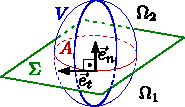
\includegraphics{./img/boundary.pdf}
    \end{center}
    Sprungbedingung für die Normalenableitung des Potentials:\\
    \begin{eqnarray*}
        \epsilon_1\frac{\partial \Phi}{\partial n}\big|_1 - \epsilon_2\frac{\partial \Phi}{\partial n}\big|_2 = \sigma_{\ir int} \text{ auf }\Sigma\\
    \end{eqnarray*}
    An Grenzflächen gibt es Flächenladung $\sigma:$ \\
    $Q = \lim\limits_{h \ra 0} \int_V \rho \diff V = \int_A \sigma \diff \vec a$\\

    Die Tangentialkomponente des E-Feldes\\ und die Normalkomponente des B-Feldes sind stetig
    \begin{eqnarray*}
        \vec D_2 \vec n - \vec D_1 \vec n = \sigma_{\ir int} \\
        \vec B_2 \vec n - \vec B_1 \vec n = 0 \\
        \vec E_1 \times \vec n - \vec E_2 \times \vec n = 0 \\
        \vec H_2 \times \vec n - \vec H_1 \times \vec n = \vec j
    \end{eqnarray*}
    Brechungsgesetz für elektrische Feldlinien (2 Isolatoren): \\
    \begin{eqnarray*}
        \frac{\tan \alpha_1}{\tan \alpha_2} = \frac{\varepsilon_1}{\varepsilon_2}
    \end{eqnarray*}
    Gleiches gilt für $\vec j = 0$ auch für das $\vec B$ bzw. $\vec H$-Feld
\end{sectionbox}
\subsection{Randwertprobleme der Potentialtheorie}
Homogenes Randwertproblem: Beide Grenzen haben Potential 0.\\
Zu lösen ist die \textsc{Poisson}-Gleichung $\div(\varepsilon \nabla \Phi) = -\rho$ auf $\interior \Omega$:\\
\begin{tabular*}{\columnwidth}{@{\extracolsep\fill}llll@{}}
    Nr. & RWP & Randbedingungen auf $\partial \Omega$ & Lösung\\
    1. & Dirichlet & $\Phi\big|_{\partial\Omega} = \Phi_D$ & eindeutig $\Phi \in \mathcal C^2$\\[0.5em]
    2. & Neumann & $\frac{\partial \Phi}{\partial \vec n}\Big|_{\partial\Omega} = F_N$ & eindeutig $(\Phi + C) \in \mathcal C^2$\\[0.5em]
    3. & Gemischt & $\left( \Phi + k \frac{\partial \Phi}{\partial \vec n}\right)\Big|_{\partial\Omega} = F_N$ & eindeutig $\Phi \in \mathcal C^2$\\
\end{tabular*}
Mit Richtungsableitung $\frac{\partial \Phi}{\partial \vec n}\big|_{1/2} = \lim\limits_{\vec r - \vec r_0 \ra 0} \vec n(\vec r_0)  \nabla\Phi(\vec r)$ \quad $\vec r \in \Omega_{1/2}$\\
\\
Lösungsansatz: $\Phi = \Phi^{(0)} + \varphi$\\
$\Phi^{(0)}:$ erfüllt hom. DGL und inhom. RB\\
$\varphi:$ erfüllt inhom. DGL und hom. RB\\
\\
In den meisten Elektrostatischen Problemen gilt $\rho = 0$, da sich die Ladung nur auf den Grenzflächen von Leitern befindet und nicht im Gebiet $\Omega$ in dem die Lösung von $\Phi$ gesucht wird.\\
In der Praxis sind die meisten RWPs gemischt, wie Leiterkontakte oder Wärmeleitung\\

Mehrelektroden-Kondensator Q-RWP:\\
$\div(\varepsilon \nabla \Phi) = 0$ in $\interior \Omega$ und $\int_{\partial \Omega_l} \varepsilon \frac{\partial \Phi}{\partial \vec n} \diff \vec a = Q_l$ und  besitz bis auf eine additive Konstante eine eindeutige Lösung

\subsubsection{Spektralzerlegung}
Lösungsverfahren:\\
\begin{enumerate}
    \item Ansatz: $\Phi = \Phi^{(0)} + \varphi$\\
          Finde hinreichend glatte Funktion $\Phi^{(0)}$ welche inhomogene Randgleichungen erfüllt
    \item Finde Eigenfunktionen von $\varphi$: $f=-\div(\varepsilon \nabla \vec b_\nu) = \lambda_\nu \vec b_\nu$\\
          Es gilt $\lambda_\nu > 0$.
    \item Ansatz $\varphi(\vec r) = \sum_{\nu = 1}^\infty \alpha_\nu b_\nu(\vec r)$\\
          Bestimmung der Entwicklungskoeffizienten: $a_\nu = \frac{<b_\nu|f>}{\lambda_\nu} = \frac{1}{\lambda_\nu}\int_\Omega b_\nu * f dv$\\
    \item Spektraldarstellung: $G(\vec r, \vec r') = \sum_{\nu = 1}^\infty b_\nu (\vec r) \frac{1}{\lambda_\nu} b_\nu (\vec r')^*$\\
\end{enumerate}



\subsection{Greenfunktion $G$}
Def: Lösung des RWP mit hom. Randbed. und Störung $\rho(\vec r) = \delta(\vec r - \vec r')$ (Einheitspunktladung bei $\vec r'$)\\
Poissongleichung $\Delta\varphi = -\frac{\rho}{\varepsilon_0}$ wird durch das Coulomb-Integral gelöst.
Allg. Lösung: $\Phi(\vec r) = \varphi(\vec r)+\psi(\vec r) = \int_\Omega G(\vec r, \vec r')\rho(\vec r') \diff^3 \vec r' + \psi(\vec r)$\\
für $\varepsilon(\vec r) = \varepsilon$: $\psi(\vec r) = -\varepsilon\iint_{\partial V^{(D)}}\left[\dfrac{\partial G(\vec r, \vec r')}{\partial\vec n'}\Phi_D(\vec r')\right]\diff a'+\varepsilon\iint_{\partial V^{(N)}}\left[G(\vec r, \vec r')\dfrac{\partial\Phi_N(\vec r')}{\partial n'}\right]\diff a'$
\\
Beispiel Punktladung: $G_{\text{Vac}}(\vec r, \vec r') = \frac{1}{4 \pi \varepsilon} \frac{1}{\norm{\vec r - \vec r'}}$

\subsubsection{Spektralzerlegung mit Greenfunktion}
Problem: \boxed{- \lpo \varphi = \tilde{f}}

\begin{itemize}
    \item Sperationsansatz für die Eigenfunktionen: \\
          $b(\vec r) = b_1 (x_1) b_2(x_2) b_3(x_3)$
    \item $- \frac{b_1''(x_1)}{b_1 (x_1)} - \frac{b_2''(x_2)}{b_2 (x_2)}  - \frac{b_3''(x_3)}{b_3 (x_3)} = \lambda$
    \item Aufteilen des Problems: \\
          $- \frac{b_1''(x_1)}{b_1 (x_1)} = \lambda_1$ \\
          $- \frac{b_2''(x_2)}{b_2 (x_2)} = \lambda_2$ \\
          $- \frac{b_3''(x_3)}{b_3 (x_3)} = \lambda_3$
    \item Lösungsansatz für $b_1, b_2, b_3$: \\
          $b_j (x_j) = A_j \sin(k_j x_j) + B_j \cos (k_j x_j)$ mit $k_j = \sqrt{\lambda_j}$
    \item $\Ra B_j = 0$ und $k_j L_j = n_j \pi$
    \item Eigenfunktionen lauten: \\
          $b_j ( x_j ) = A_j \sin (n_j \frac{\pi}{L_j} x_j)$
    \item Normiere die Eigenfunktionen: \\
          $1 \overset{!}{=} \int \limits_0^{L_k} b_j (x_j)^2 \diff x_j$
\end{itemize}

Die Greenfunktion lautet nun: \\
$G(\vec r, \vec r') = \sum \limits_{n_1, n_2 , n_3 \in \mathbb N} b_{n_1 n_2 n_3} (\vec r ) \frac{1}{\lambda_{n_1}\lambda_{n_2}\lambda_{n_3}} b_{n_1 n_2 n_3} (\vec r' )$
%TODO S.52 Skript Lösungen der Laplace-Glg.
\subsection*{Spiegelladungsmethode}
Konstruktion eines Ersatzproblems durch Spiegelung der negierten Ladung an einer ebenen leitenden Randfläche\\
%TODO S.63 Bild
\begin{align*}
    G_{\text{Halb}}(\vec r, \vec r_0) = \frac{1}{4 \pi \varepsilon} \left( \frac{1}{\norm{\vec r - \vec r_0}} - \frac{1}{\norm{\vec r - \vec r_0^*}}\right)
\end{align*}
analog für Winkelräume. Eventuell müssen die gespiegelten Ladungen wieder gespiegelt werden (möglicherweise unendlich oft), bis sich alles ausgleicht.

\subsection*{Multipolentwicklung}
Coulomb-Integral: $\Phi(\vec r) = \int_{\R^3} G_{\ir vac}(\vec r, \vec r')\rho(\vec r') \diff^3 \vec r' = \frac{1}{4\pi\varepsilon_0}\int_{\R^3}  \frac{\rho(\vec r)}{\abs{\vec r - \vec r'}}\diff v'$\\
Vereinfachung der Integraldarstellung durch Taylorentwicklung des Integralkerns $\frac{1}{\abs{\vec r - \vec r'}}$ unter der Annahme $\abs{\vec r'} < \abs{\vec r}$:
$\Phi(\vec r) = \frac{1}{4\pi\varepsilon_0}\frac{1}{r}Q + \frac{1}{4\pi\varepsilon_0}\frac{\vec r  \vec p}{r^3} \mp \hdots$


\subsection{Stationäre Ströme und RWP}
Einflüsse: Drift, Diffusion, Hall-Effekt, Seebeck-Effekt\\
Drift-Diffusionsmodell:\\
\boxed{ \begin{array}{rll} \vec j = & \underset{\text{Driftstrom}}{\sum\limits_{\alpha = 1}^N |q_\alpha| n_\alpha \mu_\alpha \vec E} & - \underset{\text{Diffusionsstrom}}{\sum\limits_{\alpha = 1}^N q_\alpha D_\alpha \nabla n_\alpha} + \\[2em] + & \underset{\text{Halleffekt}}{\sum\limits_{\alpha = 1}^N \sigma_\alpha R_\alpha^H \vec \j_\alpha \times \vec B} & \underset{\text{Seebeck}}{-\sum\limits_{\alpha = 1}^N \sigma_\alpha P_\alpha \nabla T} \end{array}
}\\
$-\sum\limits_{\alpha = 1}^N \sigma_\alpha P_\alpha \nabla T$

%$\sum\limits_{\alpha = 1}^N \sigma_\alpha R_\alpha^H \vec \j_\alpha \times \vec B



\section{Orthogonalreihenentwicklung}
Was möchten wir lösen? Poisson ($\Delta\Phi(\vec{r}) = -\frac{\rho (\vec{r})}{\epsilon}$) oder Spezialfall Laplace ($\Delta\Phi(\vec{r}) = 0$).\\
\begin{tablebox}{lcc}
    \ctrule
    &Poisson ($\rho \neq 0$)&Laplace ($\rho = 0$)\\\cmrule
    \makecell[l]{homogene\\Randwerte}   &
    \makecell[l]{$\Phi = \iiint\limits_VG(\vec{r},\vec{r}')\rho(\vec{r}')d^3r$\\$\varphi$: Greenfunktion lösen für\\ Ergebnis und Orthogonal-\\reihenentwicklung}&
    $\Phi = 0$
    \\\cmrule
    \makecell[l]{inhomogene\\Randwerte} &
    \makecell[l]{Ansatz: $\Phi = \varphi + \psi$\\(Randwertprobleme)\\$\psi$: Dirichlet/Neumann RWB,\\$\varphi$: Greenfunktion}&
    \makecell[l]{Orthogonal-\\reihenentwicklung}
    \\\cbrule
\end{tablebox}

\subsection{$\varphi$ bestimmen}
Laplaceoperator: lineare Summe von gewichteten Teillösungen ist wieder eine Lösung.\\
$\Rightarrow$ Ansatz: $\Phi(\vec{r}) = \sum\limits_{n=1}^{\infty}\alpha_nb_n(\vec{r})$ ($\alpha_n$: Gewichtung, $b_n$: Eigenfunktion von $\Delta$: $f''=bf$)\\
$\Delta b_n(\vec{r})=\begin{cases}\lambda_nb_n(\vec{r}), &\text{Poisson}\\0, &\text{Laplace}\end{cases}$\\
$\Rightarrow \Delta\Phi(\vec{r}) = \begin{cases}\sum\limits_{n=1}^{\infty}a_n\lambda_nb_n(\vec{r})=-\frac{\rho}{\epsilon}, &\text{Poisson}\\0, &\text{Laplace}\end{cases}$\\
\textbf{Seperationsansatz: $\Delta b_n(\vec{r})$ lösen}
\begin{enumerate}
    \item $b_n(\vec{r}) = b_1(x)b_2(y)b_3(z) \hat{=} X(x)Y(y)Z(z)$
    \item in den Ansatz einsetzen $\rightarrow$ gewöhnliche DGL
    \item Randwerte einsetzen $\rightarrow$ mit homogenen RW anfangen
    \item Konstanten zusammenfassen $\rightarrow$ z.B. $A_n B_n \mapsto \tilde{A}_n$
\end{enumerate}
\subsection{Lösen von Poisson-Gleichung}
$-\Delta b_n = \lambda_ib_n$ mit $b_n=b_1(x)b_2(y)b_3(z)$
\begin{align*}
    -b_1''b_2b_3-b_1b_2'b_3-b_1b_2b_3''                       & =\lambda_ib_1b_2b_3                                            \\
    -\dfrac{b_1''}{b_1}-\dfrac{b_2''}{b_2}-\dfrac{b_3''}{b_3} & =\lambda_i \Rightarrow \dfrac{-b_i''(x_i)}{b_i(x_i)}=\lambda_i
\end{align*}
$\Rightarrow b_i''(x_i)+b_i(x_i)\lambda_i \stackrel{!}{=} 0$ \qquad (1)\\
\textbf{Ansatz für DGL: } $b_i(x_i)=A_i\sin(x_ik_i)+B_i\cos(x_ik_i)$ \quad in (1)\\
$\dfrac{\partial^2}{\partial x_i^2}(A_i\sin(k_ix_i)+B_i\cos(k_ix_i))+\lambda_i(A_isin(k_ix_i)+B_icos(k_ix_i)) \stackrel{!}{=} 0$\\
$(A_i\sin(k_ix_i)+B_i\cos(k_ix_i))(\lambda_i-k_i^2)\stackrel{!}{=}0$\\
$\Rightarrow \lambda-k_i^2=0 \Leftrightarrow$ \boxed{\lambda_i=k_i^2} \boxed{\sqrt{\lambda_i}=k_i }\\
\textbf{Randwerte für $b_i$}
Ansatz: $A_i\sin(k_i 0)+B_i\cos(k_i 0)$\\
$b_i(0)=0=B_i$\\
$b_i(L_i)=A_i\sin(k_iL_i)=0\Rightarrow$ \boxed{k_i=\frac{n\pi}{L_i}}$, n\in \mathbb{N}$\\
\textbf{Orthonormierung}
$\int\sin^2(u)du=\frac{1}{2}$\\
Ansatz: $1 = \int\limits_0^{L_i}b_i^2(x_i)dx_i\Rightarrow A_i=\sqrt{\frac{2}{L_i}}$\\
einsetzen für $b$: $n=3$\\$\Rightarrow b_{n_1n_2n_3}(x_i)=\dfrac{\sqrt{2}^3}{\sqrt{L_1L_2L_3}}\prod\limits_{i=1}^3\sin\left(\dfrac{n_i-\pi}{L_i}x_i\right), n\in\mathbb{N}$\\
    einsetzen in $G(\vec{r},\vec{r}')$: $G(\vec{r},\vec{r}') = \sum\limits_{n=1}^{\infty}b_n^*(\vec{r}')\frac{1}{\lambda_n}b_n(\vec{r})$
    \subsection{Orthogonalreihenentwicklung zu Laplace}
    \textbf{Beispiel}: Randwerte überall 0, außer bei $\Phi(x_1,x_2,x_3=L_3)=V(x,y)$\\
    \textbf{Ansatz}: $-\frac{b_1''}{b_1} -\frac{b_2''}{b_2}-\frac{b_3''}{b_3}=0$\\
$\Rightarrow \lambda_1+\lambda_2+\lambda_3 = 0$ mit hom. RW $\Leftrightarrow \lambda_3 = -(\lambda_1+\lambda_2)$\\
$k_3 = \sqrt{\lambda_3} = \j\beta$\\
$b_{1,2,3}(0)\Rightarrow B_{1,2,3}=0$\\
$b_{1,2}(L_{1,2})=0\Rightarrow K_{1,2}=\frac{n_{1,2}\pi}{L_{1,2}}$\\
$\Rightarrow b_{1,2}(x_{1,2}) = A_{1,2}\sin\left(n_{1,2}\frac{\pi}{L_{1,2}}x_{1,2}\right)$\\
$\Rightarrow \lambda_3 = -(\lambda_1+\lambda_2) = -\beta < 0, K_3=\sqrt{\lambda_3}=\sqrt{-(\lambda_1+\lambda_2)}$\\
$b_3(x_3)=A_3\sinh(\beta x_3)$ ($j$ steckt in $A$)\\
    \textbf{Ansatz für DGL:}\\
$b_{n_1,n_2}(\vec{r}) = A_{n_1}A_{n_2}A_3\sin\left(\frac{n_1\pi}{L_1}x_1\right)\sin\left(\frac{n_2\pi}{L_2}x_2\right)\sinh(\beta x_3)$\\ \\
    Ersetzen von $A_{n_1}A{n_2}A_{n_3} = A_{n_1n_2}$, da $A_3 = \ir const$:\\
$\Phi(\vec{r}) = \sum\limits_{n_1=1}^{\infty}\sum\limits_{n_2=1}^{\infty}b_{n_1,n_2}(\vec{r})$\\
    \boxed{
        \begin{array}{lcl}
            \Phi(x_1,x_2,x_3=L_3)=V(x,y)= \\
            \sum\limits_{n_1=1}^{\infty}\sum\limits_{n_2=1}^{\infty}A_{n_1n_2}\sin\left(\frac{n_1\pi}{L_1}x_1\right)\sin\left(\frac{n_2\pi}{L_2}x_2\right)\sinh(\beta x_3)
        \end{array}
    }
    \textbf{1D Fall:} $V(x)=\sum\limits_{n=1}^{\infty}A_n\sin\left(\frac{n\pi}{L}x\right)$\\
    Bestimmung von $A_{\textcolor{orange}{2}}$:\\
$V(x) = \int\limits_0^{L}\sin\left(\frac{\textcolor{orange}{2}\pi}{L}x\right)\diff x = \overset{\ir =0}{\overbrace{A_1\int\limits_0^{L}\sin\left(\frac{1\pi}{L}x\right)\sin\left(\frac{\textcolor{orange}{2}\pi}{L}x\right)\diff x}} + \overset{\ir =L/2}{\overbrace{A_2\int\limits_0^{L}\sin\left(\frac{2\pi}{L}x\right)\sin\left(\frac{\textcolor{orange}{2}\pi}{L}x\right)\diff x}} + \overset{\ir =0}{\overbrace{...}}, \overset{\delta_{\ir nm}: n\neq m = 0}{\text{da Orthogonalitätsbed.}}$\\
$V(x) = \int\limits_0^{L}\sin\left(\frac{n\pi}{L}x\right)\sin\left(\frac{m\pi}{L}x\right)\diff x = \begin{cases}0, &m\neq n\\\frac{L}{2}, &m=n\end{cases}$\\
$\Rightarrow$ \boxed{ A_n = \frac{2}{L} \int_0^L V(x)\sin\left(\frac{n\pi}{L}x\right)\diff x}
    \section{Kompaktmodelle}
    Modellierung als Netzwerk ohne Wellenausbreitung.\\
    Vorraussetzungen:\\
    \begin{enumerate}
    \item Räumlich begrenzte Funktionsblöcke:\\
    lokalisierte Schnittstellen (leitende Verbindungen, geführte elektromagnetische Felder)\\
    \item Quasistationär zeitveränderlich:\\
    Konzentriertheitshypothese: $\lambda >> d$.\\
    Knoten: ideal leitend, überall gleiches Potential.\\
    Zweige: flusserhaltend, gerichtete Spannung.\\
    \end{enumerate}

    \boxed{\lambda = \frac{c_0}{f}}


    \subsection{Kirchoffsche Gesetze}
    \boxed{ \sum U_i = U_{\ir ind} } \qquad \boxed{ \sum I_i = - \dot Q_K }\\

    \subsection{Kapazitive Speicherelemente}
    Mehrelektroden Kondensatoranordnung $\rightarrow$ Modellierung als Netzwerk von kapazitiven Zweipolen.\\
    Plattenkondensator: \\
$\vec E = \frac{Q}{\varepsilon_0A}\vec\e$ \qquad $U = \int_0^d \vec E\diff\vec r = \frac{Q}{\varepsilon_0A}d$
    \begin{itemize}
    \item Kapazitätsmatrix:\\
$C_{kl} = \int\limits_\Omega \nabla \Phi_k \varepsilon \nabla \Phi_l \diff^3 r = -\int\limits_{\partial\Omega_k} \epsilon \vec n \nabla \Phi_l d\vec a$ (k,l = 0, ..., N)\\
$\ma C$ symmetrisch, positiv semi-definit, nicht invertierbar, Zeilen- und Spaltensumme null\\
    \item Reduzierte Kapazitätsmatrix:\\
$\ma C_0: \ma C$ um 0. Zeile und 0. Spalte abgeschnitten\\
$\vec U_0 = \mat{ V_1 - V_0 \\ s \\ V_N - V_0 }$ \quad $\vec Q_0 = \ma C_0\vec U_0$ \quad $\ma C_0$ invertierbar\\

    \end{itemize}

    \subsection{Induktive Speicherelemente}
$u_k(t) = -u_{\text{ind,k}}(t) + r_ki_k(t)$\\
    Transformatorgleichung: $u_k(t) = r_ki_k(t)+\sum_{l=1}^N L_{\ir kl} \frac{\diff i_l}{\diff t}$\\
    Kopplungsinduktivität: $M = k\sqrt{L_1L_2}$\\
$\quad\Rightarrow U_1=L_1\dot{I}_1 + M\dot{I}_2\qquad U_2 = M\dot{I}_1+L_2\dot{I}_2$\\
    Neumannsche Formel: $L_{\text{kl}} = \frac{\mu}{4\pi}\int_{C_k}\int_{C_l} \frac{d\vec s'  d\vec s}{\abs{\vec r - \vec r'(s)}} = \frac{\partial^2W_{\ir mag}}{\partial i_k\partial i_l}$ \\
$L_{\text{kl}} : \begin{cases}\text{Selbstinduktionskoeffizient}, k=l\\\text{Gegeninduktionskoeffizient}, k \neq l\end{cases}$\\
$\ma L$ symmetrisch, positiv definit



    \begin{tabular*}{\columnwidth}{@{\extracolsep\fill}ll@{}} \trule
    Kapazität & Induktivität\\
$\vec Q = \ma C \vec U$ & $\vec \Phi_M = \ma L \vec i$\\
$W_{\text{el}} = \frac{1}{2}\vec U_0\vec Q_0 = \frac{1}{2}\vec V^T\ma C\vec V$ & $W_{\ir mag} = \frac{1}{2} \vec I^\top \ma L \vec I$\\
    & $\boxed{ W_{\ir mag} = \frac{1}{2} \int\limits_{\R^3} \vec j  \vec A \diff^3 r }	$
    \end{tabular*}\\
    \columnbreak

    % .:: Elektromagnetische Wellen
    %=======================================================================
    \section{Elektromagnetische Wellen}
    Transportieren Feldenergie mit Lichtgeschwindigkeit. $\varepsilon \mu c^2 = 1$\\
    Unendliche Ausbreitung mit Lichtgeschwindigkeit ohne Medium.\\
    Wechselwirkung mit der Materie.\\
    Frequenzabhängigkeit von $\varepsilon(\omega),\mu(\omega),\sigma(\omega)$\\
    Annahmen: $\rho = 0$ außer bei Antennen, keine thermischer Strom.\\

    \subsection{Beschreibung}
    \begin{tabular}{l@{\hspace{4em}}l}
    \ctrule
    Dämpfung & falls $\sigma > 0$\\
    äußere Quellen & $\vec j_0, \rho_0$\\
    \ctrule

    \end{tabular}

    6-Komponentiges, elektromagnetisches Wellenfeld:\\
$\mat{ \varepsilon \mu \frac{\partial^2}{\partial t^2} + \mu \sigma \frac{\partial}{\partial t} - \lpo } \vect{ \vec E \\ \vec H } = \vect{ - \nabla \left(\frac{\rho_0}{\varepsilon}\right) - \mu \dot{\vec j}_0 \\ \rot \vec j_0 }$
    Notwendig, aber nicht hinreichend für Maxwellsche Gleichungen. \\(Nebenbedingungen: $\varepsilon \div \vec E = \rho, \div \vec H = 0$)\\
    4-Komponentiges, elektromagnetisches Potential (falls $\sigma = 0$):\\
$\left(\Delta - \varepsilon\mu \frac{\partial^2}{\partial t^2}\right) \vect{\Phi \\ \vec A} = - \vect{\frac{\rho}{\varepsilon} \\ \mu \vec j }$

    Als Nebenbedingung muss nur die Eichbedingung erfüllt sein.\\

    homogene Wellengleichung: \boxed { \left(\frac{1}{c^2}\frac{\diff^2}{\diff t^2}-\Delta\right)\vec E = 0}

    \subsection{Eindimensionale Welle}
    Annahmen: $\sigma, \vec j_0,\rho_0 = 0 \Rightarrow \epsilon\mu \frac{\partial^2u}{\partial t^2}-\frac{\partial^2 u}{\partial x^2} = 0$\\
    Ausbreitungsgeschwindigkeit: $c = \frac{1}{\sqrt{\epsilon\mu}}$\\
    D'Alembertsche Lösung: $u(x,t) = f_1(ct-x)+f_2(ct+x)$\\
    \subsection{Dreidimensionale ebene Wellen}
    Annahhmen: $\sigma, \rho_0, \vec j_0 = 0$ \\
    Nebenbedingungen: $\div\vec E =\div \vec H = 0$ \quad $\rot \vec E = -\mu\frac{\partial\vec H}{\partial t}$ \quad $\rot \vec H = \frac{\partial\vec E}{\partial t}$\\
    \boxed{\vec k = k\vec n, \omega=kc} Dabei muss gelten: $\frac{\omega}{\abs{\vec k}} = c = \frac{1}{\sqrt{\epsilon\mu}}$\\
$\vec E(t,\vec r) = \vec E_0(\omega t-\vec k\vec r)$ mit $\vec k\vec E_0(.) = 0$\\
$\vec E_0(\vec r,t) =\frac{\vec k}{\epsilon \omega} \times \vec H_0(\vec r,t) = -Z\vec n \times \vec H_0(.)$\\
$\vec H(t,\vec r) = \vec H_0(\omega t-\vec k\vec r)$ mit $\vec k\vec H_0(.) = 0$\\
$\vec H_0(\vec r,t) =\frac{\vec k}{\mu \omega} \times \vec E_0(\vec r,t)= \frac{\vec n}{Z}\times \vec E_0(.)$\\
    Dispersionsrelation: $\omega(\vec k) = \frac{1}{\sqrt{\epsilon\mu}}\abs{\vec k}$\\
    Wellenwiderstand: $Z = \sqrt{\frac{\mu}{\epsilon}} = \frac{\abs{\vec E_0}}{\abs{\vec H_0}}$\\
    \subsubsection{Energie- und Leisungsbetrachtung}
$w_{\ir el}(t,\vec r) = w_{\ir mag}(t,\vec r) = \frac{\epsilon}{2}\vec E_0(\omega t-\vec k\vec r)^2 = \frac{\mu}{2}\vec H_0(\omega t-\vec k\vec r)^2$\\
    Leistungsflussdichte: $\vec S = \frac{1}{Z}\vec E_0^2\vec n$\\
    Energiebilanz einer elektromagnetischen Welle: $\frac{\partial w_{\ir elmag}}{\partial t} + \div \vec S = 0.$\\
    \subsection{Harmonische ebene dreidimensionale Wellen}
    \subsubsection{Linear polarisierte Wellen}
$\vec E(t,\vec r) = \vec E_0\cos(\omega t-\vec k\vec r + \varphi)$\\
$\vec H(t,\vec r) = \vec H_0\cos(\omega t-\vec k\vec r + \varphi)$\\
    \subsubsection{Elliptisch polarisierte Wellen}
$\vec E(\vec r,t) = E_{01} \cos(\omega t -\vec k\vec r + \varphi_1) \vec e_1 + E_{02} \cos(\omega t - \vec k\vec r + \varphi_2) \vec e_2$\\
    %TODO Ab hier ists noch nicht gemacht	
    Harmonische, ebene EM Wellen ($\sigma = 0$)\\

    Ellipsengleichung:\\
$\left(\frac{E_1}{E_{01}}\right)^2 + \left(\frac{E_2}{E_{02}}\right)^2 - 2\left(\frac{E_1}{E_{02}}\right)\left(\frac{E_1}{E_{02}}\right) \cos(\varphi_{02} - \varphi_{01}) = \sin^2(\varphi_{02} - \varphi_{01})$\\
    Linear: $\varphi_{02} - \varphi_{01} = n\pi$ \qquad $\frac{E_1}{E_{01}} = \pm \frac{E_2}{E_{02}}$\\
    Kreis: $\varphi_{02} - \varphi_{01} = (n+\frac{1}{2}) \pi \ \land \ E_{01} = E_{02}$ \qquad $\left(\frac{E_1}{E_{01}}\right)^2 + \left(\frac{E_2}{E_{02}}\right)^2$\\

    \subsubsection{Komplexe Darstellung}
$\vec E(t,\vec r) = \Re{\underset{\hat E_0}{\underbrace{\left(E_{\ir 01}\e^{j\varphi_1}\vec\e_1 + E_{\ir 02}\e^{j\varphi_2}\vec\e_2\right)}\e^{j(\omega t-\vec k\vec r)}}}$\\
    \subsubsection{Darstellung beliebiger EM-Wellen durch harmonische ebene Wellen}
    Annahmen: $\rho_0, \vec j_0 = 0, \sigma \geq 0$\\
    Materialgleichungen:
    \begin{itemize}
    \item $\vec D(\vec k) = \epsilon(\omega(\vec k))\vec E(\vec k)$
    \item $\vec B(\vec k) = \mu(\omega(\vec k))\vec H(\vec k)$
    \item $\vec j(\vec k) = \sigma(\omega(\vec k))\vec E(\vec k)$
    \end{itemize}
    komplexe Permittivität: $\tilde{\cx \varepsilon}(\omega) = \varepsilon(\omega) + \i \frac{\sigma(\omega)}{\omega}$\\
    komplexe Dispersionsrelation: $\omega(\vec{k})^2=\frac{1}{\tilde{\varepsilon}(\omega(\vec k))\mu(\omega(\vec k))}\vec k^2$\\
    komplexer Wellenwiderstand: $\tilde{Z}(\omega) = \sqrt{\frac{\mu(\omega)}{\tilde{\varepsilon}(\omega)}} = \frac{\tilde{k}(\omega)}{\omega\tilde{\varepsilon}(\omega)}$\\
    Fourierkoeffizienten der Feldgrößen:
    \begin{itemize}
    \item $\rot\vec E = -\frac{\partial\vec B}{\partial t} \overset{FT}{=} -j\vec k \times\hat{\vec E}(\vec k) = -j\omega\mu(\omega)\hat{\vec H}(\vec k)$, also $\vec k\times\hat{\vec E}(\vec k) = \omega(\vec k)\mu(\omega(\vec k))\hat{\vec H}(\vec k)$
    \item $\div\vec D = 0 \overset{FT}{=} -j\vec k\varepsilon(\omega)\hat{\vec E}(\vec k) = 0$, also $\vec k\hat{\vec E}(\vec k) = 0$
    \item $\rot\vec H = \vec j + \frac{\partial\vec D}{\partial t} \overset{FT}{=} \sigma(\omega)\hat{\vec E}(\vec k)+j\omega\varepsilon(\omega)\hat{\vec E}(\vec k) = j\omega\tilde{\varepsilon}(\omega)\hat{\vec E}(\vec k)$, also $-\vec k\times\hat{\vec H}(\vec k) = \omega(\vec k)\tilde{\varepsilon}(\omega(\vec k))\hat{\vec E}(\vec k)$
    \item $\div\vec B = 0 \overset{FT}{=} j\vec k\mu(\omega)\hat{\vec H}(\vec k) = 0$, also $\vec k\hat{\vec H}(\vec k) = 0$
    \end{itemize}
    inv. Dispersionsrelation: $\tilde{\cx k}(\omega) = \sqrt{\tilde{\varepsilon}(\omega)\mu(\omega)}$\\
    \subsubsection{Räumlich gedämpfte ebene EM-Welle in Leitern}
$\tilde{\cx k}(\omega) = \underset{\text{Phasenmaß}}{\beta(\omega)} - \i \underset{\text{Dämpfungsmaß}}{\alpha(\omega)}$\\
    Näherung: $\sigma(\omega) \gg \omega\varepsilon(\omega)$\\
$\alpha(\omega) = \beta(\omega) = \sqrt{\frac{\sigma(\omega)\mu\omega}{2}} = \frac{2\pi}{\lambda}$\\
    Eindringtiefe: $\Delta z(\omega) = \sqrt{\frac{2}{\sigma(\omega)\mu\omega}}$\\
    Abklingverhältnis: $\e^{-\lambda\alpha}$\\
    Skin-Effekt: Abschirmverhalten von leitenden Medien gegen das Eindringen von EM-Wellen
    \subsection{Einfall ebener elektromagnetischer Wellen auf ebene Materialgrenzschichten}
    Aufteilung der EM-Welle in reflektierenden und transmittierenden Anteil\\
    einfallend: $\vec H_h(\vec r) = \vec H_{\ir h0}\e^{-j\vec k_h\vec r}$, \qquad $\vec E_h = Z_1\vec H_h \times \e_{\ir kh}$\\
    reflektierend: $\vec H_r(\vec r) = \vec H_{\ir r0}\e^{-j\vec k_r\vec r}$, \qquad $\vec E_h = Z_1\vec H_h \times \e_{\ir kh}$
    transmittierend: $\vec H_D(\vec r) = \vec H_{\ir D0}\e^{-j\vec k_D\vec r}$, \qquad $\vec E_h = Z_2\vec H_h \times \e_{\ir kh}$
    %TODO Bild Skript S.163
    Reflexionswinkel gleich Einfallswinkel: $\alpha_h = \alpha_r$\\
    Brechungsgesetz (Snellius): $k_1\sin\alpha_h = k_2\sin\alpha_D$\\
$(\vec H_h + \vec H_r) \times \vec n = \vec H_D \times\vec n \qquad (\vec E_h + \vec E_r)\times n = \vec E_D \times \vec n$
    \textbf{E-Feld $\parallel$ Einfallsebene:} Einfallende Welle nennt sich TM-Welle\\
    %TODO Bild Skript S.165
    Reflexionskoeffizient: $r_{\parallel} = \frac{\hat E_r}{\hat E_h} = \frac{\hat H_r}{\hat H_h} = \frac{Z_2\cos\alpha_D - Z_1\cos\alpha_h}{Z_2\cos\alpha_D + Z_1\cos\alpha_h}$\\
    Transmissionskoeffizient: $t_{H\parallel} = \frac{\hat H_D}{\hat H_h} = \frac{2Z_1\cos\alpha_h}{Z_2\cos\alpha_D+Z_1\cos\alpha_h}$\\
$t_{E\parallel} = \frac{\hat E_D}{\hat E_h} = \frac{Z_2}{Z_1}t_{H\parallel}$\\
    \textbf{E-Feld $\perp$ Einfallsebene:} Einfallende Welle nennt sich TE-Welle\\
    Reflexionskoeffizient: $r_\perp = \frac{\hat E_r}{\hat E_h} = \frac{\hat H_r}{\hat H_h} = \frac{Z_2\cos\alpha_h-Z_1\cos\alpha_D}{Z_2\cos\alpha_h+Z_1\cos\alpha_D}$\\
    Transmissionskoeffizient: $t_{E\perp} = \frac{\hat E_D}{\hat E_h} = \frac{2Z_2\cos\alpha_h}{Z_2\cos\alpha_h+Z_1\cos\alpha_D}$\\
$t_{H\perp} = \frac{\hat H_D}{\hat H_h} = \frac{Z_1}{Z_2}t_{E\perp}$\\
    \subsection{Abstrahlung von EM-Wellen im freien Raum}
    Maxwellsche Gleichungen in zeitharmonischen Feldern:
    \begin{itemize}
    \item $\rot\vec E = -\j\omega\vec B = -\j\omega\mu_0\vec H$
    \item $\rot\vec H = \j\omega\vec D + \vec j_0 = \j\omega\varepsilon_0\vec E+\vec j_0$
    \item $\div\vec E = \frac{1}{\epsilon_0}\div\vec D = \frac{\rho_0}{\varepsilon_0}$
    \item $\div\vec H = \frac{1}{\mu_0}\div\vec B = 0$
    \end{itemize}
    Helmholtz-Gleichung: $\Delta\vec A + \j\omega\varepsilon_0\mu_0\vec A = -\mu_0\vec j_0$\\
    Vereinfachung durch eingeprägte Dirac-Impuls Stromdichte der Form: $\vec j_0^D(\vec  r) = \hat I_0\Delta l\vec\e_z\delta(\vec r)$\\
$\Rightarrow$ \textbf{Hertzscher-Dipol} mit Dipolmoment $I_0\Delta l$ mit $\vec A(\vec r) = \hat I_0\Delta l\mu_0\frac{\e^{-\j k_0r}}{4\pi r}\vec\e_z$\\
    %TODO Bild Skript S. 169
    \subsection{Elektromagnetische Wellenleiter}
    Alle Verbindungen zwischen elektrischen und elektronischen Bauteilen oder Systemen sind Wellenleiter (bei niedrigen Frequenzen vernachlässigbar).\\
    Wellenausbreitungseffekte ab $\frac{1}{10}\lambda \rightarrow$ Vermeidung von Reflexionen und Mehrwegeausbreitungseffekten\\
    Translationsinvarianz des Wellenleiters in z-Richtung $\rightarrow$ Feldtypen der Form:
    \begin{align*}
        \vec E(x,y,z) = \vec E_0(x,y)\e^{\pm\gamma} \\
        \vec H(x,y,z) = \vec H_0(x,y)\e^{\pm\gamma}
    \end{align*}
$\gamma = \j\beta$: verlustloser Wellenleiter\\
$\gamma = \alpha$: Dämpfungstypen (evaneszente Moden)\\
    Wellentypen können eine \textbf{untere Grenzfrequenz} aufweisen, ab der sie ausbreitungsfähig sind\\
    Existiert unterhalb einer bestimmten Grenzfrequenz noch eine einziger Wellentyp $\Rightarrow$ \textbf{Grundmode / Fundamentalmode} (i.d.R. bei Leitungen TEM-Welle).\\
    Koaxialleitung:
    \begin{align*}
        \vec E(\vec r) = \frac{\hat U_0}{\ln\left(\frac{D}{d}\right)}\frac{1}{r}\vec\e_r\e^{-\j kz}       \\
        \vec H(\vec r) = \frac{\hat I_0}{\ln\left(\frac{D}{d}\right)}\frac{1}{r}\vec\e_\varphi\e^{-\j kz} \\
        \underset{\textbf{Leitungswellenwiderstand}}{\frac{\hat U_0}{\hat I_0} = Z_L = 60\Omega\sqrt{\frac{\mu_r}{\varepsilon_r}}\ln\left(\frac{D}{d}\right)}
    \end{align*}
    mit $D$: Innendurchmesser, $d$: Außendurchmesser\\

    Rechteckhohlleiter:
    \begin{align*}
        H_z(\vec r) = -\hat H_0\cos\left(\frac{\pi}{a}x\right)\e^{-\j\beta z)}                                     \\
        H_x(\vec r) = -\j \frac{\beta}{\beta_c}\frac{\pi}{a}\hat H_0\sin\left(\frac{\pi}{a}x\right)\e^{-\j\beta z} \\
        H_y(\vec r) = 0\qquad E_x(\vec r) = 0                                                                      \\
        E_y(\vec r) = \j \frac{\omega\mu}{\beta_c}\frac{\pi}{a}\hat H_0\sin\left(\frac{\pi}{a}x\right)\e^{-\j\beta z}
    \end{align*}
    mit $\beta_c = \omega_c\sqrt{\varepsilon\mu} = \frac{2\pi}{\lambda_c}$: Cut-off-Wellenzahl, $\omega_c$: Cut-off-Kreisfrequenz, $\lambda_c = 2a$: Cut-off-Wellenlänge\\
    Ausbreitungsfähig für Kreisfrequenzen oberhalb von Ausbreitungskonstante: $\beta = \sqrt{\omega^2\varepsilon\mu-\beta_c^2}$

    \begin{description}
    \item[statisch:] Keine Veränderung über die Zeit $\frac{\partial}{\partial t} = 0$
    \item[stationär:] zeitliche Veränderung, aber keine Wellenausbreitung
    \item[Quasi-Stationär:] Zeitliche Veränderungen sind so langsam, dass sie als statisch angenommen werden $\frac{\partial}{\partial t} \approx 0$
    \item[Normalgebiet:] zusammenhängend, beschränkt, mit glattem lipschitstetigem Rand
    \item[Lipschitstetig:] irgendwas zwischen stetig und differenzierbar
    \end{description}
$\mathcal L_2(\Omega) = \iset{f:\Omega \ra \C}{\int_\omega |f(\vec r)|^2 \diff^3 \vec r < \infty }$\\

    \section{Nützliches Wissen $\rot E \equiv 0$}
    Elektrostatik heißt $\frac{\partial \vec D}{\partial t} = 0$, $\vec j = 0$ und Magnetostatik $\frac{\partial \vec B}{\partial t} = 0$ sonst spricht man von Elektrodynamik
\subsection{Komplexe Zeiger}
\begin{itemize}
    \item $\underline U = U_1 + jU_2$
    \item $\underline U = \hat U (\cos\varphi + j\sin\varphi)=\hat U e^{j\varphi}$
    \item $\varphi = \arctan(\frac{U_2}{U_1})$
\end{itemize}

\begin{equation*}
    \cos(x) = \sin(x + \frac{\pi}{2}) \quad \sin(x) = \cos(x - \frac{\pi}{2})
\end{equation*}

\subsection{Konstanten}
\begin{tabular*}{\columnwidth}{@{\extracolsep\fill}ll@{}} \trule
    Lichtgeschwind. & $c = \frac{1}{\sqrt{\varepsilon_0 \mu_0}} = \SI{299 792 458}{\meter\per\second}$\\
    Elektr. Feldkonst. & $\varepsilon_0 = \SI{8.854 188e-12}{\farad\per\meter}$\\
    Magn. Feldkonst. & $\mu_0 = 4\pi \times \SI{e-7}{\henry\per\meter}$\\
\end{tabular*}

\subsection{Mathematik}
\hspace{-20pt}
\scalebox{0.77}
{
    $\begin{array}{c|c|c|c|c|c|c|c|c|c|c|c}
            x    & 0 & \pi / 6            & \pi / 4            & \pi / 3           & \pi / 2 & \frac{2}{3}\pi    & \frac{3}{4}\pi     & \frac{5}{6}\pi      & \pi & \frac{3}{2}\pi & 2 \pi \\ \hline
            \sin & 0 & \frac{1}{2}        & \frac{1}{\sqrt{2}} & \frac{\sqrt 3}{2} & 1       & \frac{\sqrt 3}{2} & \frac{1}{\sqrt{2}} & \frac{1}{2}         & 0   & -1             & 0     \\
            \cos & 1 & \frac{\sqrt 3}{2}  & \frac{1}{\sqrt 2}  & \frac{1}{2}       & 0       & -\frac{1}{2}      & -\frac{1}{\sqrt 2} & -\frac{\sqrt 3}{2}  & -1  & 0              & 1     \\
            \tan & 0 & \frac{\sqrt{3}}{3} & 1                  & \sqrt{3}          &         & -\sqrt{3}         & -1                 & -\frac{1}{\sqrt{3}} & 0   &                & 0     \\
        \end{array}$
}
$r=|z|=\sqrt{a^2+b^2}\quad\varphi=\arg(z)=\begin{cases}+\arccos \left( \frac{a}{r}\right),  & b\ge0   \\  -\arccos \left( \frac{a}{r}\right), & b<0\end{cases}$



\label{LastPage}
\end{document}